\documentclass[conference,10pt]{IEEEtran}
\IEEEoverridecommandlockouts
% The preceding line is only needed to identify funding in the first footnote. If that is unneeded, please comment it out.
\usepackage{cite}
\usepackage{ctex}
\usepackage{amsmath,amssymb,amsfonts}
\usepackage{algorithmic}
\usepackage{graphicx}
\usepackage{textcomp}
\usepackage{xcolor}
\usepackage{float}
\usepackage{subfigure}
\def\BibTeX{{\rm B\kern-.05em{\sc i\kern-.025em b}\kern-.08em
    T\kern-.1667em\lower.7ex\hbox{E}\kern-.125emX}}
\begin{document}

\title{Towards Adversarially Robust Object Detection}

\author{\IEEEauthorblockN{
		% 1\textsuperscript{st} 
		承子杰}
	\IEEEauthorblockA{\textit{dept. AMSS(数学与系统科学研究院)} \\
		\textit{of CAS (中国科学院)}\\
		chengzijie22@mails.ucas.ac.cn\\
		202228000243001}}
\maketitle

\section{主要内容}
目标检测是计算机视觉中较为基础的研究方向之一,在无人驾驶等领域具有广泛的应用。最近的一些研究指出一些蓄意设计的对抗性样本对于目标检测器的性能会产生严重影响,但还未有研究涉及如何提高检测器的鲁棒性。为此,本文作者分析了对目标检测器不同的攻击类别,希望从中找出它们的共同点,从而提出一种对抗训练方法来提高检测器的鲁棒性。最后作者在 PASCAL-VOC 和 MS-COCO等数据集上进行大量实验,证明了该方法的有效性。
\section{目标检测问题与攻击分析}
目标检测任务将一张图像$x\in[0,255]^n$作为输入,输出$K$个目标预测$\{p_k,b_k\}^K$,其中 $p_k\in\mathbb{R}^C$ 表示在$C$个类别上的预测概率,$b_k=[x_k,y_k,w_k,h_k]$ 表示预测目标的包围盒。最后使用NMS方法作为后处理移除冗余检测来获得最后结果,其基本流程可见图\ref{fig1}。
\begin{figure}[H]
	\centering
	
\includegraphics[scale=0.3]{figure/fig1.png}
	\caption{目标检测器架构}
	\label{fig1}
\end{figure}

若我们设$\theta$ 为检测器参数,$L$为损失函数,$f(x)$为目标检测器,则模型训练目标可表示为
$$
\min\limits_\theta L(f_\theta(x),\{y_k,b_k\})
$$
在实际计算中,我们通常将上述损失函数分开表示为分类损失与位置损失,即可表示为
$$
\min\limits_\theta (L_{cls}(f_\theta(x),\{y_k,b_k\})+L_{loc}(f_\theta(x),\{y_k,b_k\}))
$$
从上述分析可以看出,目标检测可以分解为分类与位置检测两个子任务,虽然使用损失函数不同,但两者共享base-net进行特征提取,本质可以看成一个多任务学习问题。

\begin{figure}[H]
	\centering
	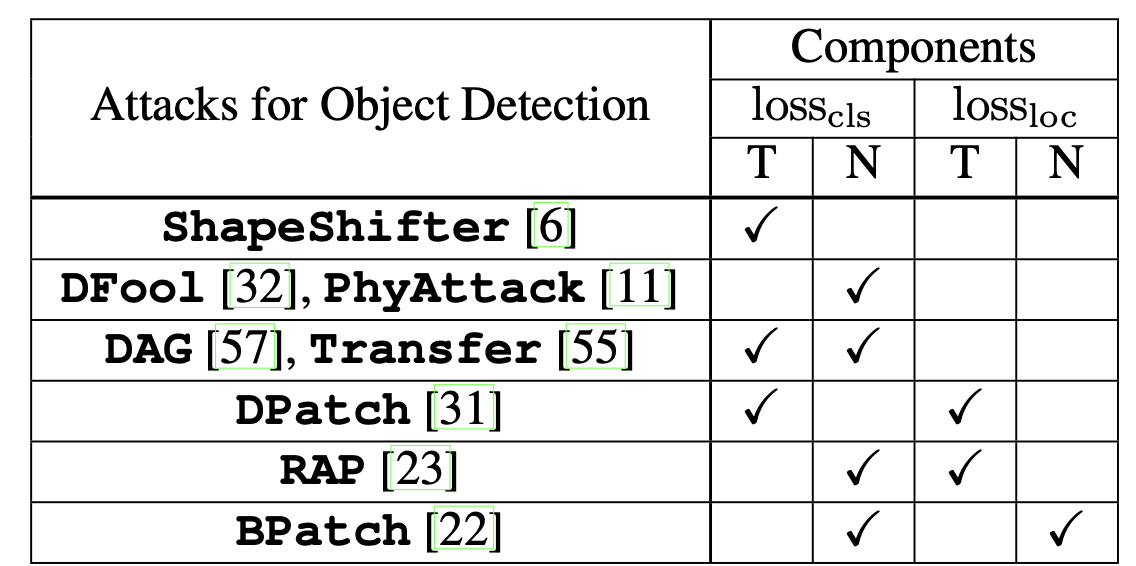
\includegraphics[scale=0.3]{figure/fig2.png}
	\caption{不同攻击分类}
	\label{fig2}
\end{figure}
根据上述检测器的设计框架,作者认为虽然攻击的方法有很多种,但设计原则都是利用单个任务损失函数的变体或其组合来实现对检测器进行攻击。为此,作者将一些常见的攻击进行了分类(对检测类别进行攻击和对检测位置进行攻击),见图\ref{fig2}。同时根据图\ref{fig1},作者认为对单个损失函数攻击能对整个检测器产生影响主要基于以下两个原因:
\begin{itemize}
	\item 由于base-net是分类与位置检测的共享网络,对base-net的弱点攻击会导致在两个任务上性能均下降。
	\item 由于最后分类与位置检测会被 NMS 耦合到一起,单个任务会影响最后结果。
\end{itemize}

\section{面向攻击的鲁棒检测}
受前一小节的启发,作者从任务丢失和任务梯度未对齐两个方面分析单任务损失对检测器鲁棒性的影响。

在任务丢失角度,作者认为由于base-net的存在,两个任务是相互影响的。对一个任务的攻击必然会影响base-net的特征提取,进而导致另一个任务性能的下降。为证明这一个观点,作者采用控制变量法。在考虑分类时,将定位因子边缘化,从而将问题转化为多类别分类任务;在考虑定位时,可以将类别信息边缘化,从而转化为类别未知下的目标检测问题。具体实验中,我们采用NMS之前的结果进行性能衡量,并采用PDG方法进行攻击。同时我们认为当锚框与标注数据的IoU>0.5时该锚框是正样本。在分类任务中,主要关心锚框的分类精度;在定位任务中,主要关心的是包围盒与标注样本的平均IoU。实验结果如图\ref{fig3} 所示。
\begin{figure}
	\centering
	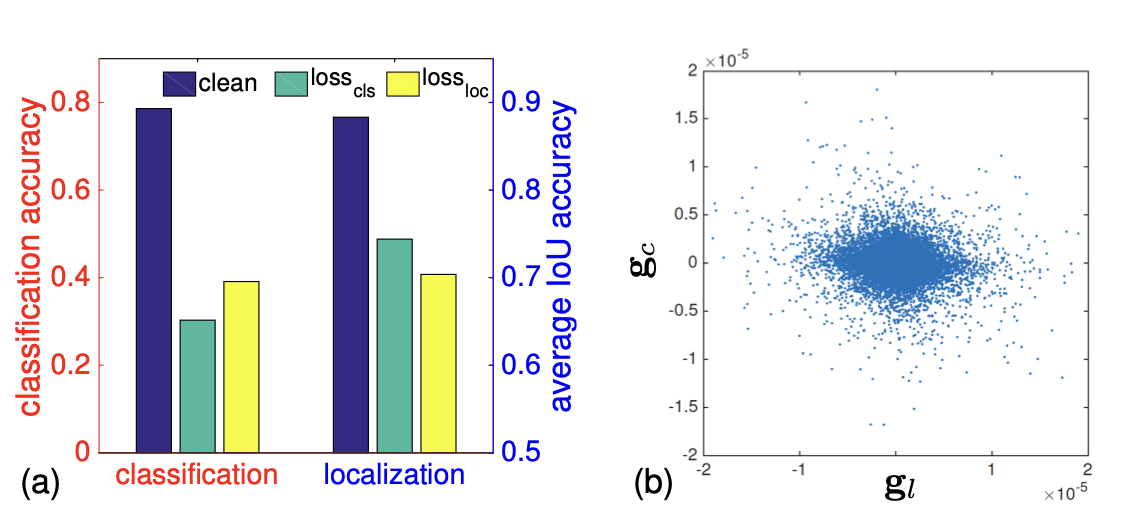
\includegraphics[scale=0.3]{figure/fig3.png}
	\caption{任务损失对检测器鲁棒性实验}
	\label{fig3}
\end{figure}
图a结果可以说明两个任务确实是相互影响,证实了作者的观点。

对于任务梯度未对齐,作者认为两个任务的梯度存在一定的共同方向,但并没有完全对齐,从而导致任务梯度的错位,这可能会混淆后续的对抗性训练。为此作者画出了两个任务损失函数梯度的逐点梯度图(图\ref{fig3}(b))进行进一步分析。通过分析可以发现两个明显问题:
\begin{itemize}
	\item 两个任务的梯度大小不相等(未呈球形),从而存在任务不平衡的问题。
	\item 两个任务的梯度方向也不一致(未呈对角线),从而存在任务梯度冲突的可能性。
\end{itemize}
\begin{figure}[H]
	\centering
	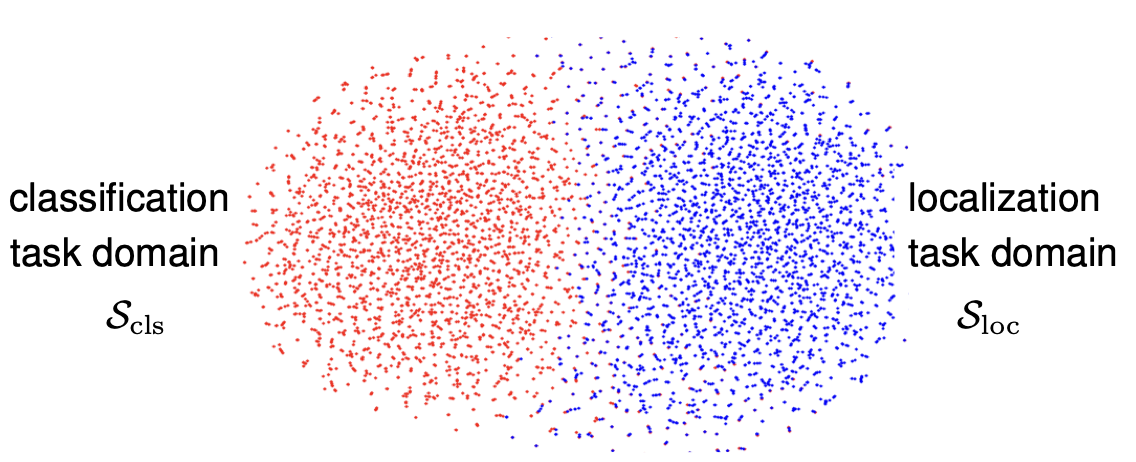
\includegraphics[scale=0.3]{figure/fig4.png}
	\caption{两个任务的梯度域}
	\label{fig4}
\end{figure}

最后,给定单一干净的图像$x$,作者画出了在不同对抗样本下,两个任务的梯度域(图\ref{fig4})。可以发现两个任务的梯度域并未完全分离,重合部分说明的是两个任务间的相互影响,分离部分说明的是两个任务的梯度未对齐。

基于上述分析,文章作者提出了改进的训练目标,即
$$
\min\limits_\theta[\max\limits_{\bar{x}\in S_{cls}\cup S_{loc}} L(f_\theta(\bar{x}), \{y_k,b_k\})]
$$
其中,$S_{cls}$ 和 $S_{loc}$ 分别表示每个任务的可行域,即
$$
\begin{array}[l]{l}
	S_{cls}\triangleq \{\bar{x}\vert arg\max\limits_{\bar{x}\in S_{x}} L_{cls}(f(\bar{x}), \{y_k\})\}\\
	S_{loc}\triangleq \{\bar{x}\vert arg\max\limits_{\bar{x}\in S_{x}} L_{loc}(f(\bar{x}), \{b_k\})\}\\
	S_x = \{z\vert z\in B(x,\epsilon)\cap [0,255]^n\}\\
	B(x,\epsilon) = \{z\vert \Vert z-x\Vert_\infty \leq \epsilon\}
\end{array}
$$
需要注意的是,与传统对抗性训练相比在分类上存在几个重要区别:
\begin{itemize}
	\item \textbf{存在多任务源},即有多个不同的监督源可用于对抗生成与训练。
	\item \textbf{面向任务的域约束},即引入$\bar{x}\in S_{cls}\cup S_{loc}$,将可行集约束至一个图像集,并对这个图像集的分类损失与定位损失进行最大化处理。该方法的优点是可以生成由每个任务指导的对抗样本,而不会受到任务之间的相互干扰。
\end{itemize}

最后,作者指出,如果我们将面向任务的域放宽到$S_x$,并设置与整个图像相对应的包围盒坐标,为每个图像分配一个单一的类别标签,则训练转变为分类设置下的常规对抗训练。从而,文章提出的鲁棒性检测对抗训练,就可以被认为是分类设置下常规对抗训练的一种自然的泛化。整个算法伪代码流程可见图\ref{fig5}。
\begin{figure}[H]
	\centering
	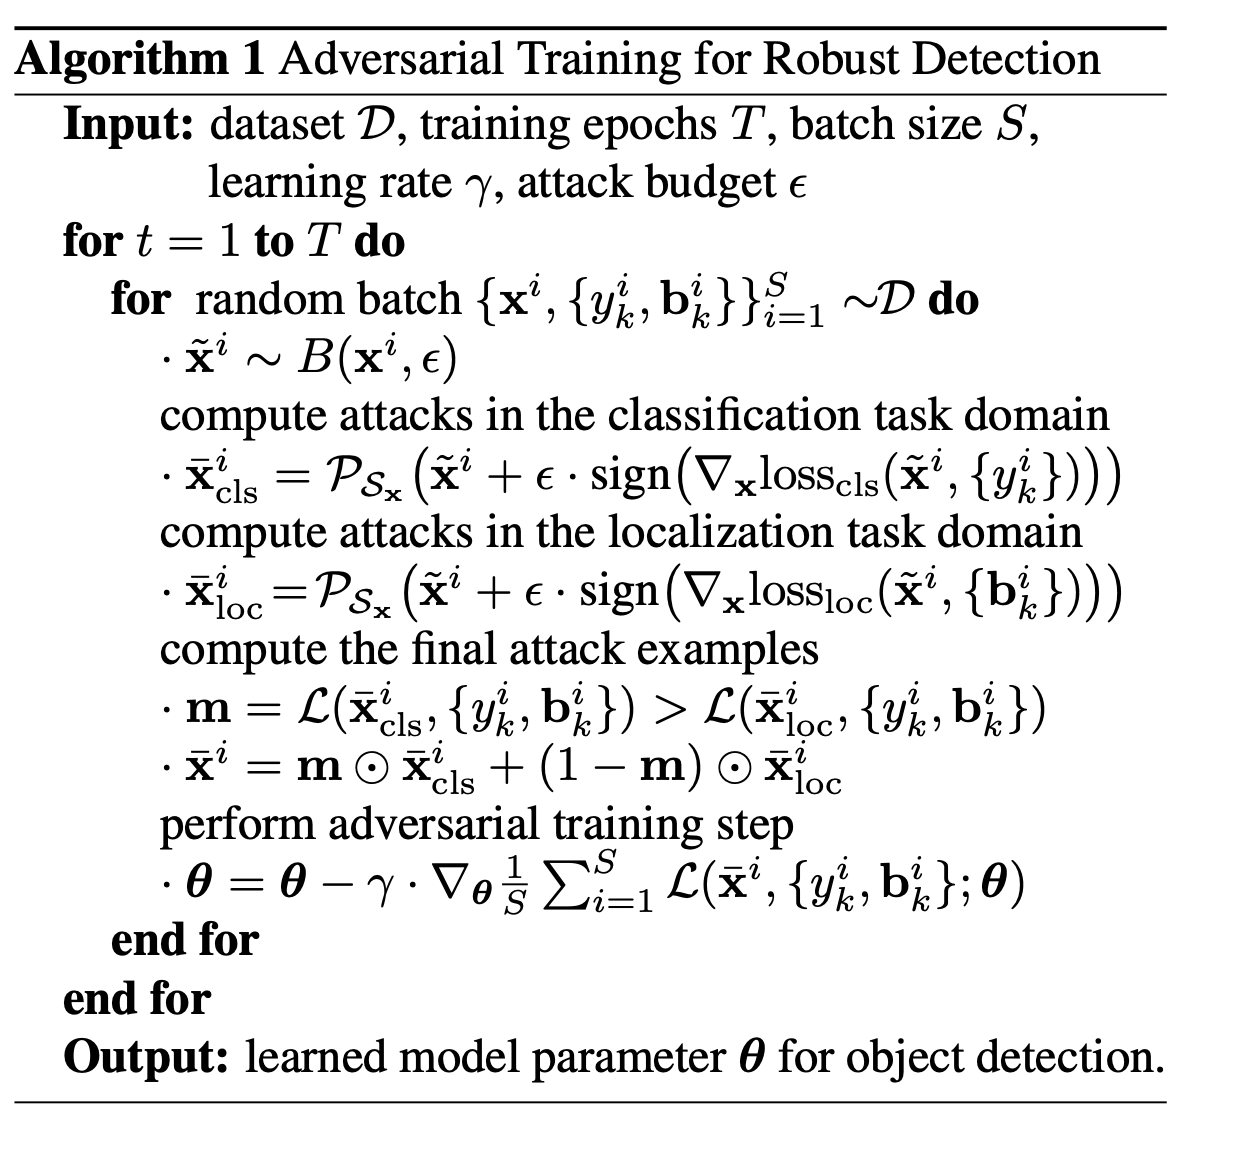
\includegraphics[scale=0.3]{figure/fig5.png}
	\caption{算法伪代码}
	\label{fig5}
\end{figure}

\section{实验结果}
作者在 PASCAL-VOC 和 MS-COCO数据集上进行训练,并使用了 DAG 和 RAP 对算法性能进行测试,测试结果见图\ref{fig6} 和图\ref{fig7}。

\begin{figure}[H]
	\centering
	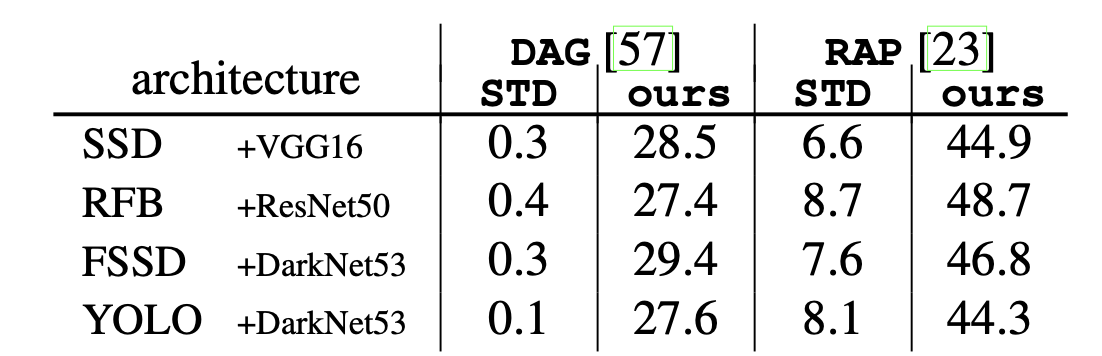
\includegraphics[scale=0.3]{figure/fig6.png}
	\caption{PASCAL-VOC 数据集上实验结果}
	\label{fig6}
\end{figure}

\begin{figure}[H]
	\centering
	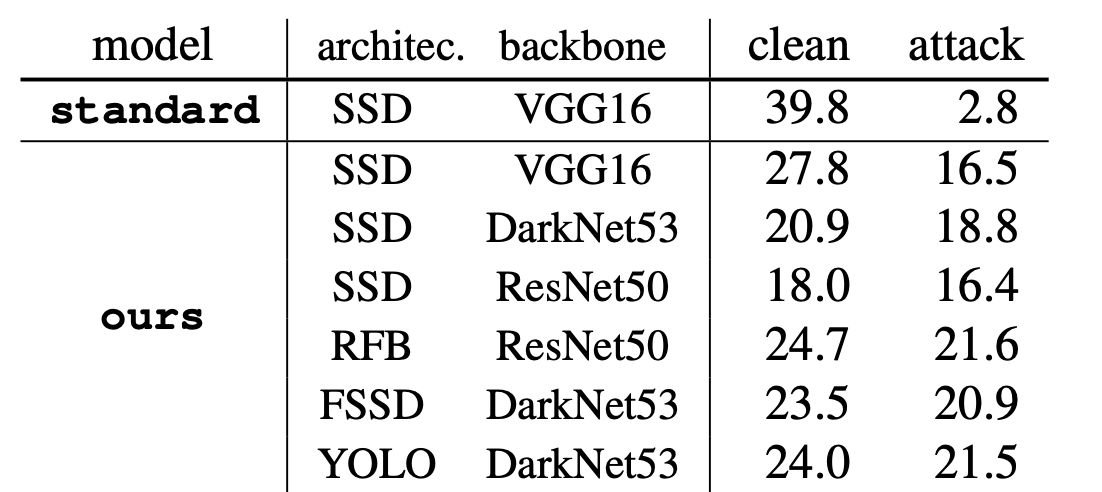
\includegraphics[scale=0.3]{figure/fig7.png}
	\caption{MS-COCO 数据集上实验结果}
	\label{fig7}
\end{figure}

通过在 PASCAL-VOC 和 MS-COCO 数据集上的实验结果表明,该算法确实提高了目标检测器的鲁棒性,这对监控场景等领域的视觉任务具有十分重要的意义。

此外作者给出了鲁棒目标检测器检测失败的例子(图\ref{fig8}),并指出具有挑战性的小图像依旧是鲁棒目标检测器难以处理的对象。作者认为对于该挑战,可能需要研究性能更优的目标探测器来解决该问题,并进一步加深对鲁棒性和目标检测架构的研究。

\begin{figure}
	\centering
	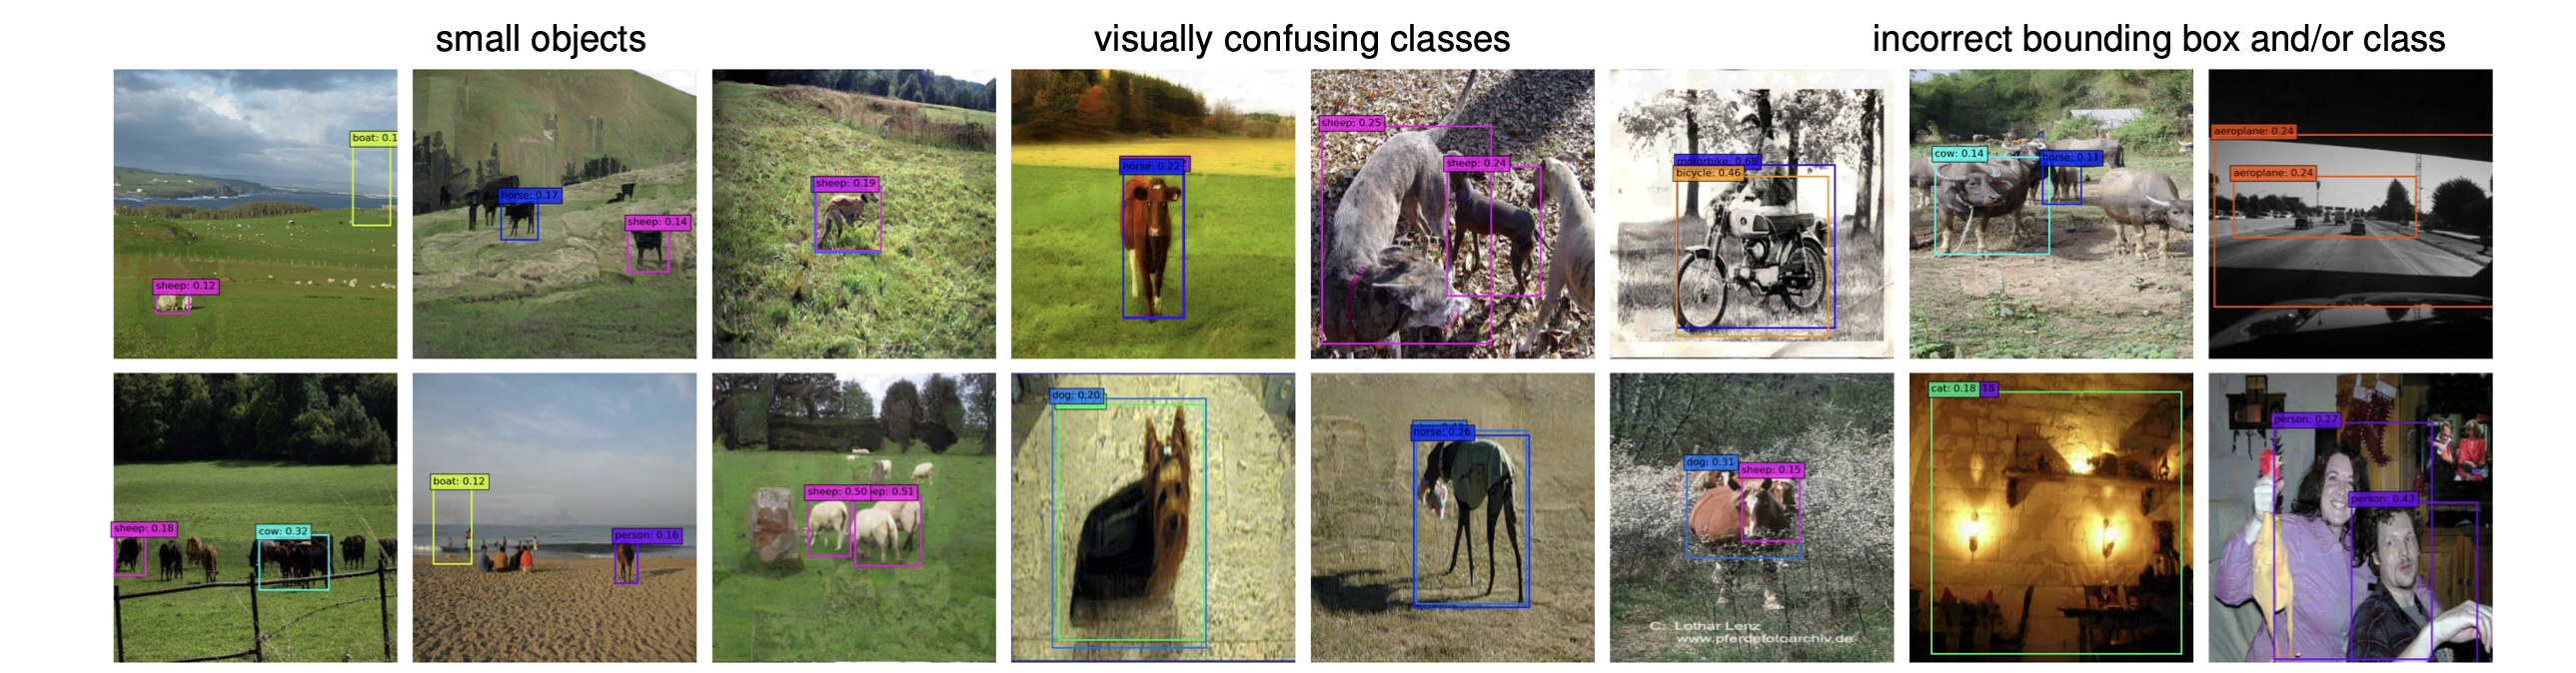
\includegraphics[scale=0.4]{figure/fig8.png}
	\caption{检测失败例子}
	\label{fig8}
\end{figure}
\section*{References}
\begin{thebibliography}{00}
\bibitem{b1} Zhang H ,  Wang J . Towards Adversarially Robust Object Detection[J]. IEEE, 2019.
\end{thebibliography}
\end{document}
